\section{JoinSystems} \label{sec:JoinSystems}

\begin{figure}[b]
  \centering
  \begin{subfigure}{0.5\textwidth} %{{{
    \begin{tikzpicture}[scale=0.8]
      \draw[very thick, ->] (0,0) -- (3.8,0) node[anchor=north] {x};
        % (0,0) node[anchor=north] {0} -- (3.8,0) node[anchor=north] {x};
      \draw[very thick, ->] (0,0) -- (0,3.3) node[anchor=east] {y};
        % (0,0) node[anchor=east] {0} -- (0,3.3) node[anchor=east] {y};
      % first system
      \draw[red, local bounding box=S1, thick]
        (1.2,0.2) rectangle (3.7,2.7);
      \node[red]
        at ({$(S1.west)!0.5!(S1.east)$} |- {$(S1.south)!0.12!(S1.north)$})
        {\small System 1};
      % second system
      \draw[blue, local bounding box=S2, thick]
        (0.2,1.2) rectangle (3.2,3.2);
      \node[blue]
        at ({$(S2.west)!0.5!(S2.east)$} |- {$(S2.south)!0.85!(S2.north)$})
        {\small System 2};
    \end{tikzpicture}
    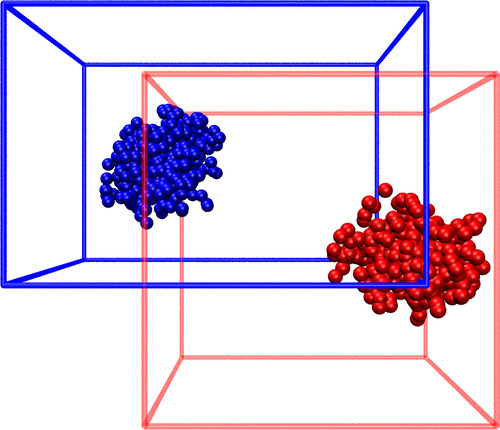
\includegraphics[height=80pt]{JoinSystems-fig_a.jpg}
    \caption{
    } \label{fig:JoinSystems-a}
  \end{subfigure} %}}}

  \begin{subfigure}{0.24\textwidth} %{{{
    \hspace{-13pt}
    \begin{tikzpicture}[scale=0.8]
      \draw[very thick, ->] (0,0) -- (3.8,0) node[anchor=north] {x};
      \draw[very thick, ->] (0,0) -- (0,3.3) node[anchor=east] {y};
      % final system
      \draw[dark-green, local bounding box=new, very thick]
        (0.2, 0.2) rectangle (3.7, 3.2);
      \fill[dark-green!15!white]
        ({$(new.west)$} |- {$(new.north)$}) rectangle
        ({$(new.east)$} |- {$(new.south)$});
      \node[dark-green]
        at ({$(new.west)!0.42!(new.east)$} |- {$(new.south)!0.9!(new.north)$})
        {New System};
      % first system
      \draw[red, local bounding box=S1, dashed, thick]
        (1.2,0.2) rectangle (3.7,2.7);
      \node[red]
        at ({$(S1.west)!0.5!(S1.east)$} |- {$(S1.south)!0.12!(S1.north)$})
        {System 1};
      % second system
      \draw[blue, local bounding box=S2, dashed, thick]
        (0.2,1.2) rectangle (3.2,3.2);
      \node[blue]
        at ({$(S2.west)!0.5!(S2.east)$} |- {$(S2.south)!0.15!(S2.north)$})
        {System 2};
    \end{tikzpicture}

    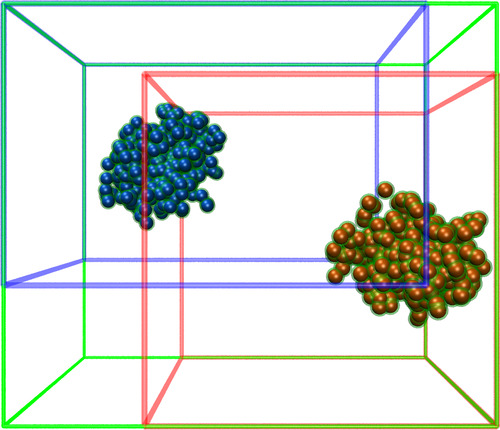
\includegraphics[height=80pt]{JoinSystems-fig_b.jpg}
    \caption{
    } \label{fig:JoinSystems-b}
  \end{subfigure} %}}}
  \begin{subfigure}{0.24\textwidth} %{{{
    \hspace{-13pt}
    \begin{tikzpicture}[scale=0.8]
      \draw[very thick, ->] (0,0) -- (3.8,0) node[anchor=north] {x};
      \draw[very thick, ->] (0,0) -- (0,3.3) node[anchor=east] {y};
      % final system
      \draw[dark-green, local bounding box=new, dashed, thick]
        (0.2, 0.2) rectangle (3.7, 3.2);
      \draw[dark-green, local bounding box=new2, thick]
        (0.95, 0.7) rectangle ++(2.0, 2.0);
      \fill[dark-green!15!white]
        ({$(new2.west)$} |- {$(new2.north)$}) rectangle
        ({$(new2.east)$} |- {$(new2.south)$});
      \draw[dark-green, dashed]
        ({$(new.west)$} |- {$(new.north)$}) --
        ({$(new.east)$} |- {$(new.south)$});
      \draw[dark-green, dashed]
        ({$(new.west)$} |- {$(new.south)$}) --
        ({$(new.east)$} |- {$(new.north)$});
      \draw[dark-green, dashed, very thick]
        ({$(new2.west)$} |- {$(new2.north)$}) --
        ({$(new2.east)$} |- {$(new2.south)$});
      \draw[dark-green, dashed, very thick]
        ({$(new2.west)$} |- {$(new2.south)$}) --
        ({$(new2.east)$} |- {$(new2.north)$});
      % first system
      \draw[red, local bounding box=S1, dashed, thick]
        (1.2,0.2) rectangle (3.7,2.7);
      % second system
      \draw[blue, local bounding box=S2, dashed, thick]
        (0.2,1.2) rectangle (3.2,3.2);
      % \draw[-latex]
      %   ({$(new.west)!0.5!(new.east)$} |- {$(new.north)!0.5!(new.south)$}) --
      %   ({$(new2.west)!0.5!(new2.east)$} |- {$(new2.north)!0.5!(new2.south)$});
      % \node[dark-green]
      %   at ({$(new.west)!0.3!(new.east)$} |- {$(new.south)!1.10!(new.north)$})
      %   {New System};
    \end{tikzpicture}

    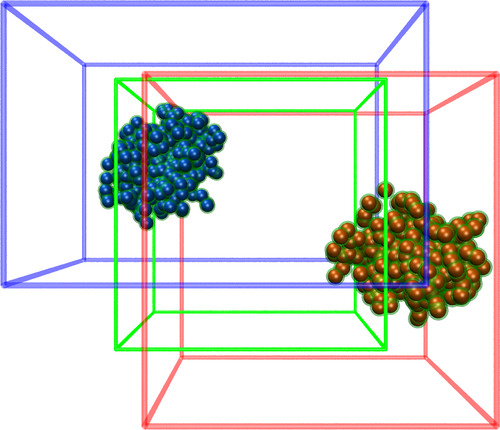
\includegraphics[height=80pt]{JoinSystems-fig_c.jpg}
    \caption{
    } \label{fig:JoinSystems-c}
  \end{subfigure} %}}}
  \begin{subfigure}{0.24\textwidth} %{{{
    \hspace{-13pt}
    \begin{tikzpicture}[scale=0.8]
      \draw[very thick, ->] (0,0) -- (3.8,0) node[anchor=north] {x};
      \draw[very thick, ->] (0,0) -- (0,3.3) node[anchor=east] {y};
      % final system
      \draw[dark-green, local bounding box=new, very thick]
        (0.95, 0.2) rectangle ++(3.0, 2.5);
      \fill[dark-green!15!white]
        ({$(new.west)$} |- {$(new.north)$}) rectangle
        ({$(new.east)$} |- {$(new.south)$});
      \draw[dark-green, dashed, very thick]
        ({$(new.west)$} |- {$(new.north)$}) --
        ({$(new.east)$} |- {$(new.south)$});
      \draw[dark-green, dashed, very thick]
        ({$(new.west)$} |- {$(new.south)$}) --
        ({$(new.east)$} |- {$(new.north)$});
      % first system
      \draw[red, local bounding box=S1, dashed, thick]
        (1.2,0.2) rectangle (3.7,2.7);
      \draw[red, dashed]
        ({$(S1.west)$} |- {$(S1.north)$}) --
        ({$(S1.east)$} |- {$(S1.south)$});
      \draw[red, dashed]
        ({$(S1.west)$} |- {$(S1.south)$}) --
        ({$(S1.east)$} |- {$(S1.north)$});
      % second system
      \draw[blue, local bounding box=S2, dashed, thick]
        (0.2,1.2) rectangle (3.2,3.2);
      \draw[blue, dashed]
        ({$(S2.west)$} |- {$(S2.north)$}) --
        ({$(S2.east)$} |- {$(S2.south)$});
      \draw[blue, dashed]
        ({$(S2.west)$} |- {$(S2.south)$}) --
        ({$(S2.east)$} |- {$(S2.north)$});
      \draw[-latex]
        ({$(S2.west)!0.5!(S2.east)$} |- {$(S2.north)!0.5!(S2.south)$}) --
        ({$(new.west)!0.5!(new.east)$} |- {$(new.north)!0.5!(new.south)$});
      % \node[dark-green]
      %   at ({$(new.west)!0.3!(new.east)$} |- {$(new.south)!1.10!(new.north)$})
      %   {New System};
    \end{tikzpicture}

    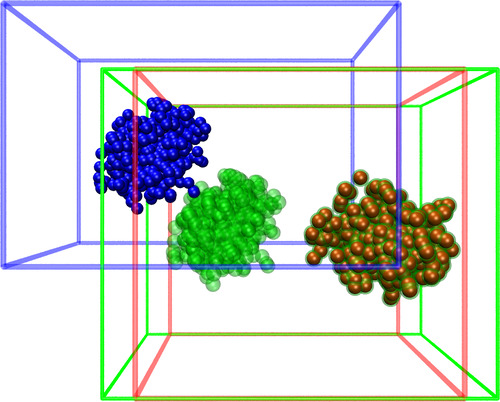
\includegraphics[height=80pt]{JoinSystems-fig_d.jpg}
    \caption{
    } \label{fig:JoinSystems-d}
  \end{subfigure} %}}}
  \begin{subfigure}{0.24\textwidth} %{{{
    \hspace{-13pt}
    \begin{tikzpicture}[scale=0.8]
      \draw[very thick, ->] (0,0) -- (3.8,0) node[anchor=north] {x};
      \draw[very thick, ->] (0,0) -- (0,3.3) node[anchor=east] {y};
      % final system
      \draw[dark-green, local bounding box=new, dashed, thick]
        (0.95, 0.2) rectangle ++(3.0, 2.5);
      \draw[dark-green, local bounding box=new2, very thick]
        (1.45, 0.45) rectangle ++(2.0, 2.0);
      \fill[dark-green!15!white]
        ({$(new2.west)$} |- {$(new2.north)$}) rectangle
        ({$(new2.east)$} |- {$(new2.south)$});
      \draw[dark-green, dashed]
        ({$(new.west)$} |- {$(new.north)$}) --
        ({$(new.east)$} |- {$(new.south)$});
      \draw[dark-green, dashed]
        ({$(new.west)$} |- {$(new.south)$}) --
        ({$(new.east)$} |- {$(new.north)$});
      \draw[dark-green, dashed, very thick]
        ({$(new2.west)$} |- {$(new2.north)$}) --
        ({$(new2.east)$} |- {$(new2.south)$});
      \draw[dark-green, dashed, very thick]
        ({$(new2.west)$} |- {$(new2.south)$}) --
        ({$(new2.east)$} |- {$(new2.north)$});
      % first system
      \draw[red, local bounding box=S1, dashed, thick]
        (1.2,0.2) rectangle (3.7,2.7);
      % second system
      \draw[blue, local bounding box=S2, dashed, thick]
        (0.2,1.2) rectangle (3.2,3.2);
    \end{tikzpicture}

    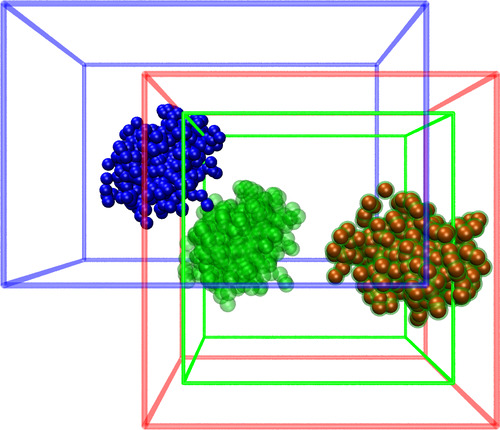
\includegraphics[height=80pt]{JoinSystems-fig_e.jpg}
    \caption{
    } \label{fig:JoinSystems-e}
  \end{subfigure} %}}}
  \caption{
    Schematic representation and corresponding snapshots illustrating
    \tt{JoinSystems} behaviour. (a) The original systems: \tt{System1.lammpstrj}
    (red) and \tt{System2.lammpstrj} (blue) in the \tt{Examples/JoinSystems}
    folder. The rest show examples of possible options (green rectangles and
    transparent balls represent the new systems): (b) no options; (c) \tt{-b 20
    20 20} option; (d) \tt{-off c c c}; (e) \tt{-b 20 20 20 -off c c c}, i.e.,
    combining (c) and (d). These new systems are in the
    \tt{Examples/JoinSystems} folder as \tt{NewSystem\_\#.lammpstrj}, where
    \tt{\#} is \tt{b}, \tt{c}, \tt{d}, or \tt{e}.
  } \label{fig:JoinSystems}
\end{figure}


This utility takes two existing systems and joins them into a single system that
contains all beads from the two coordinate files.

The second system can be offset against the first one (\tt{-off} option). In
each direction, all beads in the second system can be moved by specified
distance (only positive numbers are allowed) or moved so that the centre of that
box side is in the centre of the first box's side (use \tt{c} instead of a
number as an argument). The final box size is defined as the smallest box that
encompasses the two original boxes after the second one is moved. However, the
final box size can be redefined via the \tt{-b} option; the centre of the new
box is aligned with the centre of the original \enquote{smallest encompassing
box}. Note that no check is done whether the bead coordinates are within the new
box.

\Cref{fig:JoinSystems} illustrates the above-described behaviour (the red and
blue lines and balls represent the two original systems while the green lines
and transparent balls represent the new system). \Cref{fig:JoinSystems-b} shows
the simplest case when two systems are put into one larger system. In
\cref{fig:JoinSystems-c}, the final box size is also redefined; the positions of
the beads is unchanged, only the box size changes. Note that the absolute bead
coordinates remain unchanged only when the output coordinate file supports
defining the bounds of the simulation box; e.g., in \ltrj file, the lower and
upper bounds of the box are defined while for \vtf file, only the sidelengths of
the box are specified. Should \vtf be used as the output file, the saved
coordinates would, therefore, move so the box's origin is in the coordinate
beginning.

Using the \tt{-off c c c} option in \cref{fig:JoinSystems-d} moves the second
system (the blue one), so that the centre of its box (in all three dimensions)
lies on top of the centre of the first system's box (see the arrow in the
schematic in \cref{fig:JoinSystems-d}); coordinates of only the second system
are adjusted, changing the relative coordinates of beads from the two original
systems. If the \tt{-off} and \tt{-b} options are combined (as in
\cref{fig:JoinSystems-e}), the system created via the \tt{-off} option is then
assigned a new box size.

These examples are also provided in the \tt{Examples/JoinSystems} directory.

The output file can be any file that supports coordinates, and an extra
structure file can be created via the \tt{-o} option. Note that if an output
\vcf coordinate file is used, a \vsf structure file (with the same name except
for the extension) is also created.

\vspace{1em}
\noindent
Usage: \tt{JoinSystems <input1> <input2> <output> [options]}
\noindent
\begin{longtable}{p{0.319\textwidth}p{0.625\textwidth}}
  \toprule
  \multicolumn{2}{l}{Mandatory arguments} \\
  \midrule
  \tt{<input1>} & first input coordinate file \\
  \tt{<input2>} & second input coordinate file \\
  \tt{<output>} & output file with the new system \\
  \toprule
  \multicolumn{2}{l}{Options} \\
  \midrule
  \tt{-off <x>|c <y>|c <z>|c} & offset of the second system against the first
                                (\tt{c} to place it in the middle of the first
                                system) \\
  \tt{-b <x> <y> <z>} & side lengths of the new simulation box \\
  \tt{-o <file>} & optional output structure file \\
  \midrule
  \multicolumn{2}{l}{Other options (see the beginning of \cref{chap:Utils})}\\
  \multicolumn{2}{p{0.948\textwidth}}{As two input coordinate/structure files
    are needed, some options have 1 or 2 appended to specify which file they
    correspond to}\\
  \midrule
  \multicolumn{2}{p{0.948\textwidth}}{\tt{-i1}/\tt{-i2},
                                      \tt{-st1}/\tt{-st2},
                                      \tt{--verbose},
                                      \tt{--silent},
                                      \tt{--help},
                                      \tt{--version}}\\
  \bottomrule
\end{longtable}
